\chapter{Methodology}
\label{chap:methodology}

\section{Objectives}

The primary objective of this study is to evaluate the reliability of RSSI (Received Signal Strength Indicator) values from ESP32 Bluetooth Low Energy (BLE) beacons for determining smartphone positioning and detecting user proximity to predefined areas or points of interest (POIs) within a threshold of three meters or less. This validation is essential for ensuring that the proposed indoor localization system can accurately detect a user's presence near specific locations in museum environments.

In addition to the primary objective, the study addresses several secondary goals. First, the impact of environmental factors, such as signal interference, obstacles, and layout complexity, on localization accuracy will be assessed to ensure robustness in real-world settings. Second, the system’s responsiveness to dynamic user movements will be evaluated, focusing on latency and stability during transitions between areas and POIs. Finally, the study will compare localization accuracy across different smartphone models to determine whether variations in hardware affect the system’s reliability. These secondary objectives aim to provide a comprehensive evaluation of the system’s feasibility and generalizability.

\section{Considerations}

\subsection{Privacy and Ethical Considerations}

Protecting visitor privacy in public cultural spaces such as museums is essential, both for museums and their audiences. From an institutional perspective, it enables compliance with strict and often complex European data protection regulations (such as the General Data Protection Regulation, GDPR), while from the visitor's perspective, it fosters trust and encourages acceptance of digital technologies within the museum environment.

Traditional indoor localization systems often rely on centralized servers for data processing, which may result in sensitive location data being stored or transferred externally. This introduces legal and ethical risks, particularly when data can potentially be linked to identifiable individuals or behavioral patterns. However, recent developments in privacy-focused computing demonstrate that it is feasible to maintain localization functionality without compromising user privacy \cite{alletto_indoor_2016, spachos_ble_2020}.

In this study, privacy protection is achieved through a local-only processing model. All position computations are performed directly on the visitor’s smartphone. No user data or location history is transmitted to external systems. The server only provides static configuration data (such as beacon identifiers and positions), ensuring that all tracking and decision-making remains strictly client-side. The server data are generic, and the same for all the clients, preventing the need to identify the user. This design minimizes the risk of privacy breaches and aligns with best practices for responsible personal data processing \cite{cnil-recomendation-mobile}.

\subsection{Sustainability and Energy Efficiency}

Sustainability is an increasingly critical responsibility across public institutions, and museums are no exception. Their role in promoting sustainability is twofold: on the one hand, museums, as any actor, must address their direct environmental impact through energy-efficient infrastructure, responsible material use, and sustainable operational practices. On the other hand, they also serve as cultural and educational institutions that can foster sustainable development indirectly, by raising public awareness, inspiring behavioural change, and supporting interdisciplinary research on sustainability and climate resilience.

As emphasized by the International Council of Museums (ICOM) \cite{icom_sustainability}, museums are "perfectly positioned to address and enhance sustainability" through collaboration with communities, knowledge creation, and the promotion of planetary and societal well-being. This vision aligns with a growing movement within museums to contribute to the fulfilment of the United Nations Sustainable Development Goals (SDGs) \cite{onofri_life_2024, rodriguez_contribution_2024}.

Against this backdrop, technological solutions implemented within museum environments must be evaluated not only on performance metrics but also on their energy efficiency, environmental footprint, and alignment with institutional sustainability goals. The indoor localization system developed in this study is designed with such responsibilities in mind. Specifically, it uses ESP32-based Bluetooth Low Energy (BLE) beacons, which are known for their low power consumption and can operate for extended periods on minimal energy. Some variants may also harness solar energy, reducing battery replacement cycles and electronic waste \cite{spachos_ble_2020}.

By opting for a lightweight, low-maintenance infrastructure, this system helps minimize long-term environmental impact, while meeting technological requirements for real-time positioning. It reflects an intentional effort to align technical implementation with the broader sustainability goals increasingly embraced by cultural institutions worldwide.

\subsection{User Experience and Engagement}

Current research on indoor localization in cultural institutions has primarily focused on technical evaluation metrics such as accuracy and signal strength, with relatively few studies addressing user-centred outcomes. Visitor engagement, perception of usefulness, and interface design remain underexplored dimensions.  

For example, in \cite{alletto_indoor_2016}, personalization is introduced through a preliminary questionnaire, but systemic user feedback on the localization experience itself is largely absent. In this project, although full-scale user evaluation is beyond the scope, preliminary efforts were made to incorporate user-oriented features, such as real-time visual feedback on location and a simplified interface where the visitor can still choose to go deepen or against the automatic suggestions. Those behaviours as well as the popularity of the different areas are collected anonymously to assess both popularity and perceived added value. 

\section{Experimental Setup}

\subsection{Hardware and System Architecture}

The experimental setup comprises up to six ESP32 devices running a custom firmware that enables them to operate as BLE beacons. A picture of an ESP32 is provided at \autoref{fig:esp32}. These devices periodically broadcast BLE signals. When network access is available, they upload their position to an MQTT broker; otherwise, they function solely as standalone BLE beacons, as they don't require Wi-Fi connection to operate.

A smartphone application is responsible for collecting and processing the beacon signals. This application retrieves a list of authorized BLE beacon signatures from the MQTT broker and continuously scans for nearby devices that match these known signatures. No user data is transmitted from the smartphone to the server, ensuring privacy for both the user and other individuals within the area.

\subsection{Application Features and Localization Logic}

The smartphone application provides a real-time graphical interface that visualizes the current estimated localization for the visitor on a map. The map also shows the different areas and POIs, which are defined by the museum. The application is designed to be user-friendly and intuitive, allowing visitors to navigate the museum with ease. 

While the application is mainly thought for the visitor, it can also provide debugging and in-depth real-time analysis of the localization process for the purpose of this study. The debug map displays the static positions of the beacons, circle estimating the distance from the smartphone, a dot indicates the estimated visitor position, and finally crosses mark to show the predefined points of interest. Other graphs displays the raw RSSI, the raw distance and the filtered distance for each beacon in range.

Localization is based on RSSI-based multi-lateration. A phone is considered to be within an area when it has been detected at least twice within. Conversely, the phone is considered to have exited the area if it is subsequently detected twice at a location beyond one meter of the area. This difference between the entry and exit thresholds is implemented to prevent unstable state changes between being inside and outside an area. These threshold values have been determined based on preliminary evaluations and may be adjusted for different experimental conditions, depending on beacon placement, artwork density, and the complexity of the indoor environment.

\section{Experimental Procedure}

To systematically evaluate the performance of the system, and it's value within a museum, four distinct experiments will be conducted. These experiments focus on evaluating localization accuracy, differences in smartphone models and impact of museum layouts.

\subsection{Experimental layout}

The first experiment will take place in a designated corridor within the university, while the others are directly conducted on a floor of the museum. A picture of that floor is provided in \autoref{fig:floor-6}. ESP32 beacons will be installed at predefined locations, chosen as the best trade-off between adequate coverage of all the reference points and power socket availability within the experimental area. Participants performing the tests will execute a predefined sequence of movements, ensuring uniformity in data collection and minimizing variability caused by human movement patterns.

\begin{figure}
    \centering
    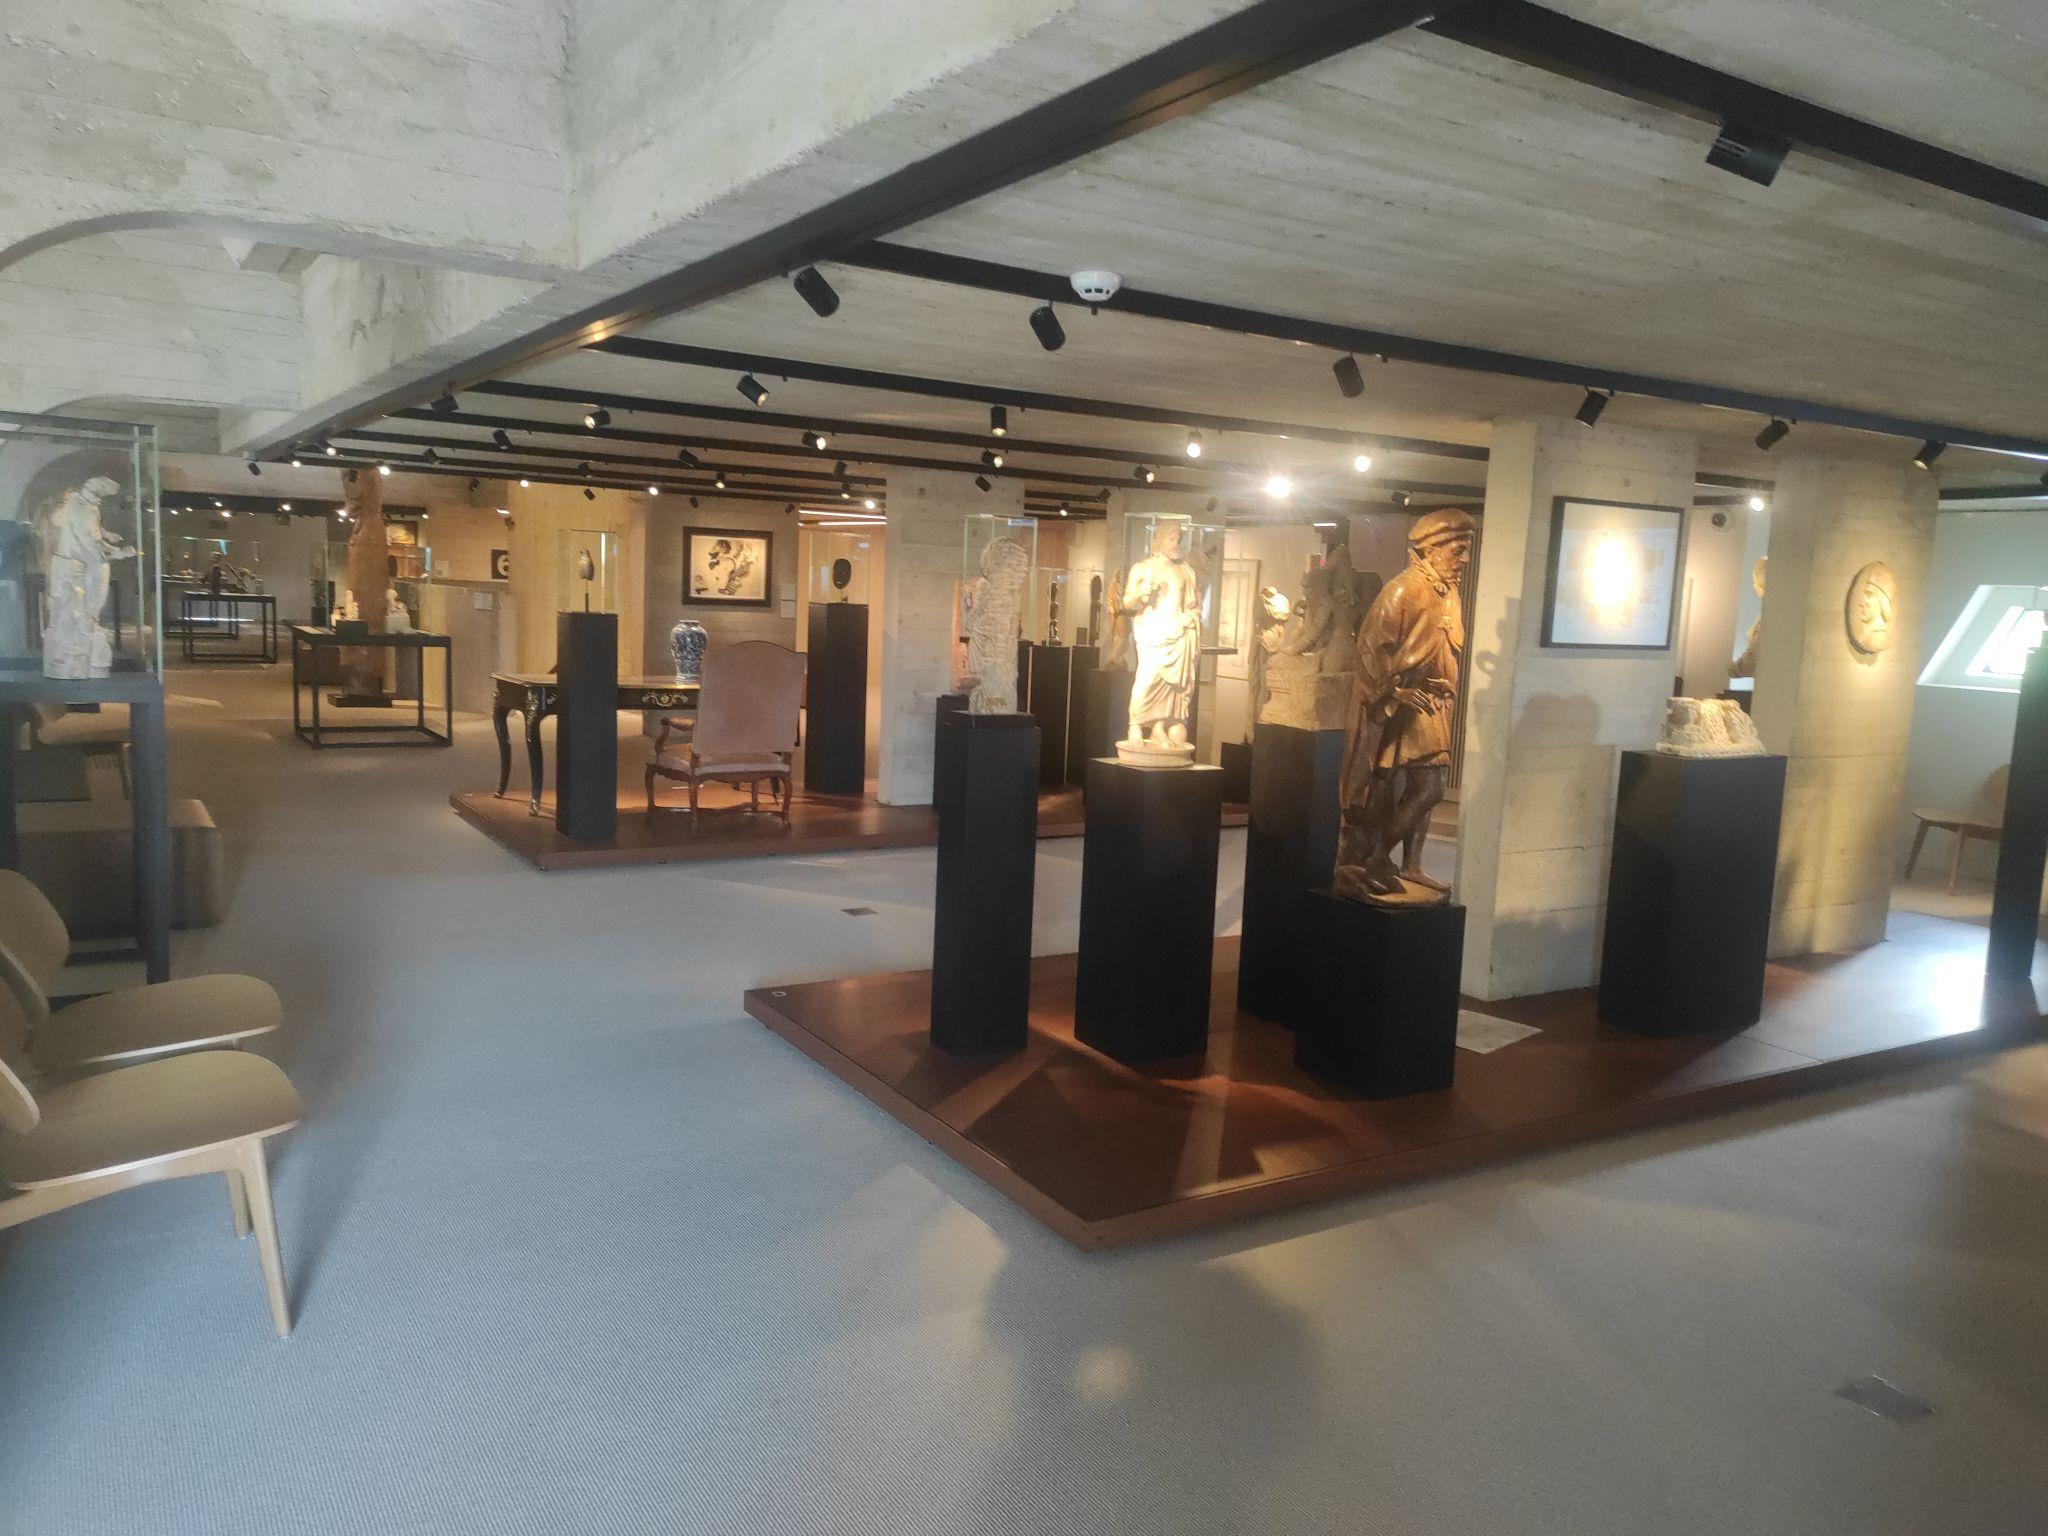
\includegraphics[width=0.75\linewidth]{assets/image-floor.jpg}
		\caption{Photo of the 6th floor of Musée L}
    \label{fig:floor-6}
\end{figure}

Localization data, including timestamps for detected entries, exits, and continuous tracking points, will be logged during all experiments. Additionally, manual records will be kept to compare the system's performance with a ground truth reference, ensuring accurate evaluation.

\subsection{Experiment 1: Localization Accuracy}
\label{exp:1_accuracy}

The first experiment focus on the beacons' data directly. It aims to calibrate the meta-parameters and analyses the precision of the distance estimation between the phone and the beacons. The experiment take place in a corridor, with no obstacle and a direct Line of Sight (LoS) between the phone and the sensors. The sensor is placed at 1.5 meters from the ground and measurements are taken at every meter, starting at "0" ($L_0$), with the phone touching the sensor, and up to 15 meters away from it ($L_{15}$). At each step, the phone take measurements for 20 seconds. Each sensor is tested with no other sensor active at the same time to minimize interferences.

\begin{figure}[H]
    \centering
    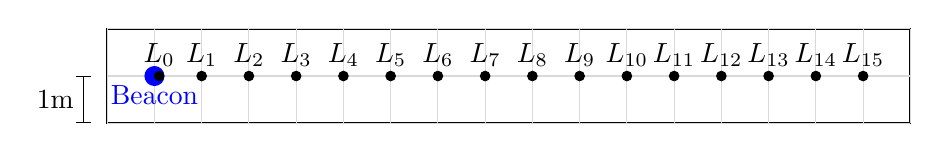
\begin{tikzpicture}[scale=0.6]
        % Room dimensions 
        \draw[thick] (0,0) rectangle (17,2);  
        % Grid (optional, for reference)
        \draw[gray!30, step=1] (0,0) grid (17, 2);
        
        % ESP32 devices (blue dots)
        \filldraw[blue] (1, 1) circle (0.2) node[below] {Beacon};

        % User positions (X marks)
        \filldraw (1.1, 1) circle (0.1) node[above] {$L_0$};
        \filldraw (2, 1) circle (0.1) node[above] {$L_1$};
        \filldraw (3, 1) circle (0.1) node[above] {$L_2$};
        \filldraw (4, 1) circle (0.1) node[above] {$L_3$};
        \filldraw (5, 1) circle (0.1) node[above] {$L_4$};
        \filldraw (6, 1) circle (0.1) node[above] {$L_5$};
        \filldraw (7, 1) circle (0.1) node[above] {$L_6$};
        \filldraw (8, 1) circle (0.1) node[above] {$L_7$};
        \filldraw (9, 1) circle (0.1) node[above] {$L_8$};
        \filldraw (10, 1) circle (0.1) node[above] {$L_9$};
        \filldraw (11, 1) circle (0.1) node[above] {$L_{10}$};
        \filldraw (12, 1) circle (0.1) node[above] {$L_{11}$};
        \filldraw (13, 1) circle (0.1) node[above] {$L_{12}$};
        \filldraw (14, 1) circle (0.1) node[above] {$L_{13}$};
        \filldraw (15, 1) circle (0.1) node[above] {$L_{14}$};
        \filldraw (16, 1) circle (0.1) node[above] {$L_{15}$};
        
        % Scale indicator
        \draw[|-|] (-0.5,0) -- (-0.5,1) node[midway, left] {1m};
    \end{tikzpicture}
    \caption{Experimental setup for the first experiment showing one beacon and all the references distances.}
    \label{fig:exp1_setup}
\end{figure}

\subsection{Experiment 2: Impact of Museum Layout and User Experience}
\label{exp:2_museum}

The second experiment combines the evaluation of the impact of the museum layout on localization results with the assessment of user experience and the system's ability to detect user presence in specific areas and provide meaningful data.

This experiment takes place directly inside the museum on the floor used for this study. All ESP32 devices are installed close to the floor, and the user keeps the smartphone in hand, in front of him. The user follows a predefined path across several locations ($L_0 \rightarrow L_1 \rightarrow~...~\rightarrow L_7$), pausing for 20 seconds at each location before moving at a walking pace to the next.

During the experiment, the application provides two layers of information to the user: an overview by section (with general information about the sections and their main art pieces), and a list of art pieces in the current section and those close to the visitor. The visitor can choose to get more information on specific pieces by interacting with the application, or simply follow the suggested path without interaction. The exact time the visitor is detected in each area is recorded alongside the classical localization data, allowing for the evaluation of both technical performance and user engagement.

\begin{figure}[H]
    \centering
    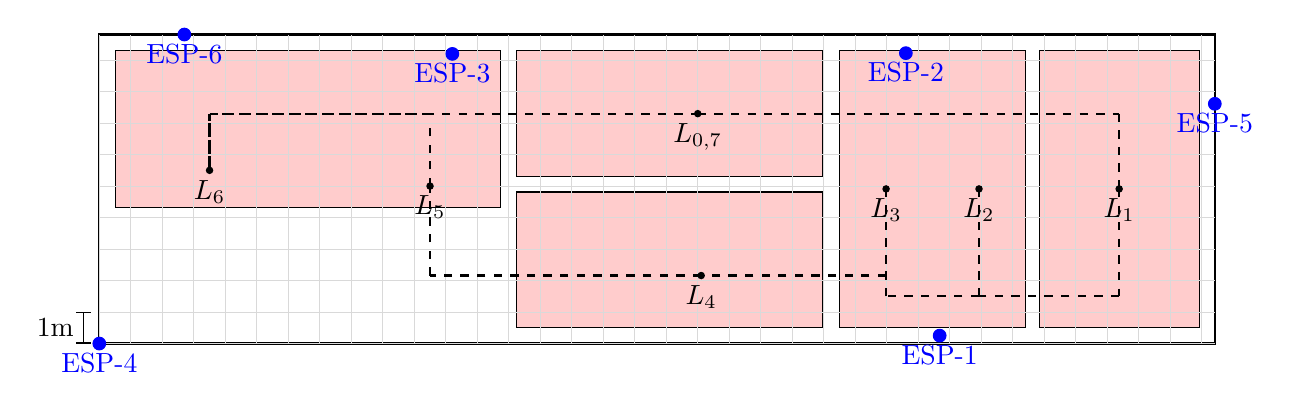
\begin{tikzpicture}[scale=0.4]
        % Room dimensions 
        \draw[thick] (0,0) rectangle (35.417, 9.812);  

        % Sections
        \draw[fill=red!20] (13.25, 5.312) rectangle (22.96, 9.312);
        \draw[fill=red!20] (29.85, 0.5) rectangle (34.917, 9.312);
        \draw[fill=red!20] (23.5, 0.5) rectangle (29.4, 9.312);
        \draw[fill=red!20] (13.25, 0.5) rectangle (22.96, 4.812);
        \draw[fill=red!20] (0.5, 4.312) rectangle (12.75, 9.312);

        % Grid (optional, for reference)
        \draw[gray!30, step=1] (0,0) grid (35.417, 9.812);

        % ESP32 devices (blue dots)
        \filldraw[blue] (26.681, 0.252) circle (0.2) node[below] {ESP-1};
        \filldraw[blue] (25.608, 9.221) circle (0.2) node[below] {ESP-2};
        \filldraw[blue] (11.209, 9.197) circle (0.2) node[below] {ESP-3};
        \filldraw[blue] (0, 0) circle (0.2) node[below] {ESP-4};
        \filldraw[blue] (35.417, 7.612) circle (0.2) node[below] {ESP-5};
        \filldraw[blue] (2.7, 9.812) circle (0.2) node[below] {ESP-6};

        % User positions
        \filldraw (19, 7.3) circle (0.1) node[below] {$L_{0,7}$};
        \filldraw (32.38, 4.91) circle (0.1) node[below] {$L_1$};
        \filldraw (27.93, 4.91) circle (0.1) node[below] {$L_2$};
        \filldraw (24.98, 4.91) circle (0.1) node[below] {$L_3$};
        \filldraw (19.11, 2.16) circle (0.1) node[below] {$L_4$};
        \filldraw (10.5, 5) circle (0.1) node[below] {$L_5$};
        \filldraw (3.5, 5.5) circle (0.1) node[below] {$L_6$};

        % Dashed lines from L0 to L1 (first X, then Y)
        \draw[dashed, thick] (19, 7.3) -- (32.38, 7.3);
        \draw[dashed, thick] (32.38, 7.3) -- (32.38, 4.91);

        % Dashed lines from L1 to L2 (first Y to 1.5, then X, then Y)
        \draw[dashed, thick] (32.38, 4.91) -- (32.38, 1.5);
        \draw[dashed, thick] (32.38, 1.5) -- (27.93, 1.5);
        \draw[dashed, thick] (27.93, 1.5) -- (27.93, 4.91);

        % Dashed lines from L2 to L3 (first Y to 1.5, then X, then Y)
        \draw[dashed, thick] (27.93, 4.91) -- (27.93, 1.5);
        \draw[dashed, thick] (27.93, 1.5) -- (24.98, 1.5);
        \draw[dashed, thick] (24.98, 1.5) -- (24.98, 4.91);

        % Dashed lines from L3 to L4 (first Y, then X)
        \draw[dashed, thick] (24.98, 4.91) -- (24.98, 2.16);
        \draw[dashed, thick] (24.98, 2.16) -- (19.11, 2.16);

        % Dashed lines from L4 to L5 (first X, then Y)
        \draw[dashed, thick] (19.11, 2.16) -- (10.5, 2.16);
        \draw[dashed, thick] (10.5, 2.16) -- (10.5, 5);

        % Dashed lines from L5 to L6 (first Y=7, then X, then Y)
        \draw[dashed, thick] (10.5, 5) -- (10.5, 7);
        \draw[dashed, thick] (10.5, 7.3) -- (3.5, 7.3);
        \draw[dashed, thick] (3.5, 7) -- (3.5, 5.5);

        % Dashed lines from L6 to L0 (first Y, then X)
        \draw[dashed, thick] (3.5, 5.5) -- (3.5, 7.3);
        \draw[dashed, thick] (3.5, 7.3) -- (19, 7.3);

        % Scale indicator
        \draw[|-|] (-0.5,0) -- (-0.5,1) node[midway, left] {1m};
    \end{tikzpicture}
    \caption{Experimental setup for the second experiment showing the beacons, reference points, and POI areas.}
    \label{fig:exp2_museum}
\end{figure}

\subsection{Experiment 3: Repeat with other phones}

The third and last experiment aim to ensure the precision of the system with multiple other phones. The exact same steps as experiment 2 are repeated, but with different phones.
